\newpage
\section{The Arbitrator Pattern for Multi-Behavior Execution}

This section describe the principle for a PASS execution that can cope with multi-behavior subjects. It is an updated version of \cite{elster:arbitrator}. The proposed interpreter is formulated using the \textit{Abstract State Machine} (ASM) concept.

\subsection{The Basic Problem}

The basic principle behind model-driven process-execution-systems (work-flow management systems) is that they use a model (most often a graph/diagram) and load it into an interpreter machine, thus forming an instance of the model. This instance, model and interpreter together, can be considered as a state machine which can be executed, or run through, until it has finished. 

One such model language is the Parallel Activity Specification Schema (PASS) introduced by Albert Fleischmann in \cite{book:Flei94}. In \cite{boerger2011interpreter} Egon Börger has presented an ASM specification for a PASS interpreter for single SBDs. 

A great challenge for model based process execution system is that the models may need to change in order to cope with change requirements in the real-life processes that they are representing and supporting. With short lived process instances that is no problem. There are cases, though, where the execution of a process instance can take weeks or months. During such duration there usually is a big chance for circumstances to arise that in turn require changing at least parts of the process model ad-hoc in order to satisfy the new needs without restarting whole process instances.
The problem is not new and described, e.g. in \cite{dadam:adept}, and research into formal requirements for such mechanism dates at least back to \cite{reichert:adeptflex}. 

An – admittedly brief – overview of the research has led to the impression that such mechanisms may although not be explicitly be applicable to PASS models and their separated-graph nature. Furthermore, the here proposed mechanism can also be used to handle the execution of multi-behavior subjects.

The basic idea to allow for an update mechanism is to incorporate a model-exchange-mechanism into the model interpreter machine. It is assumed that a mechanism exists that guaranties validity of all parts of a model in the current context and that supporting tools can be realized in a way that a multi-behavior model is valid or more specifically any diagram $D*$ (e.g. any \PASSModelElement{Extension Behavior}, \PASSModelElement{Guard Behavior}, or \PASSModelElement{Macro-Behavior}) will be a valid extension of $D$ (e.g. a \PASSModelElement{Base Behavior}) in a given currently running process context. A function $validInCurrentAmb(D*,D)$ will be the placeholder. 

The question up to discussion is whether the arbitrator pattern can be used for the task of realizing multi-behavior execution and the execution of ad-hoc extension to process models?

\subsection{The arbitrator pattern}

The arbitrator pattern stems from the field of robotics and was introduced by R.C. Arkin in \cite{arkin98behavior} to program LEGO Mindstorm robots to interact with their not predefined environment. It allows for fast and effective programming of independent robots, but was advised against for use anywhere else, but robotic.
Its basic principle assumes a robot with input and output equipment. Instead of programming a single large complex program to control the machine there is one arbitrator deciding which of many smaller behavior programs (short “behaviors”) is currently to be executed. These behaviors may contain only simple instructions like “move forward”. Which behavior is currently controlling the robot is determined by a dynamically reevaluated priority that is defined based on the sensor inputs for each behavior. As soon as external events (e.g. the robot hitting a wall) require a change, the priority is shifted and the arbitrator executes a different behavior. Behaviors can be added as required given that priority-computing-functions are included. 

\begin{figure}[htbp]
	\centering
	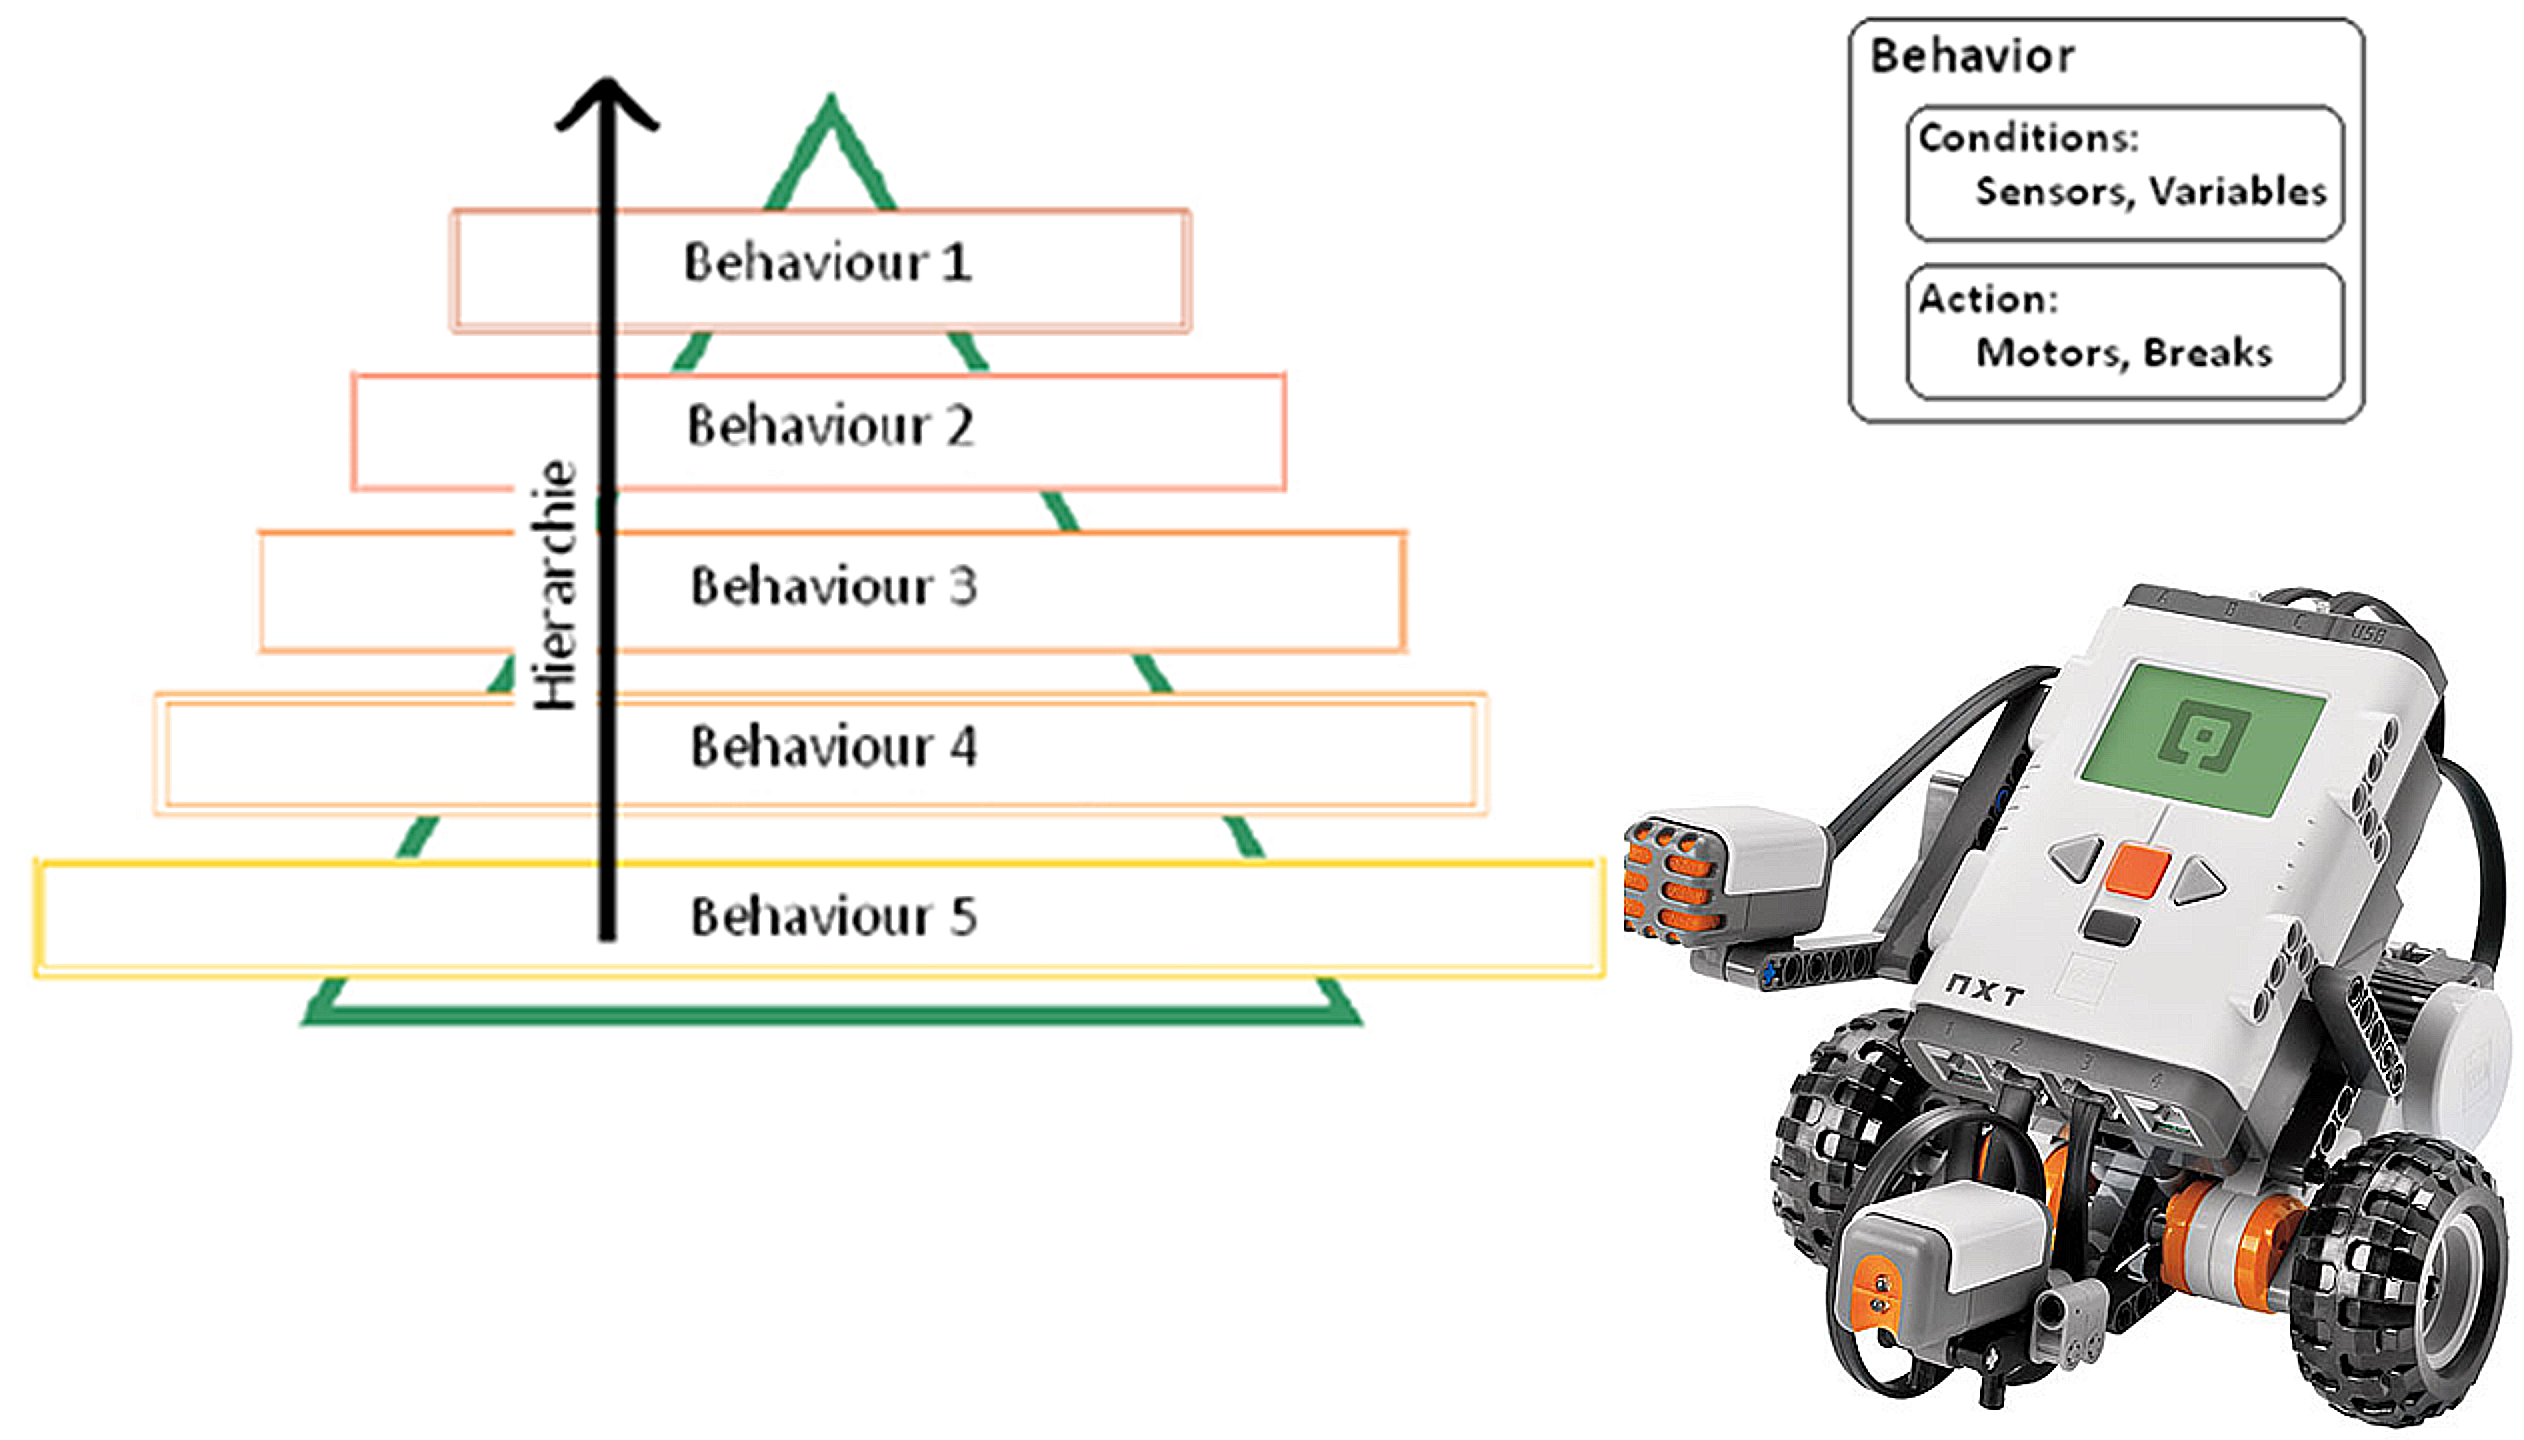
\includegraphics[width=0.8\linewidth]{Figures/Chapter5/ArbitratorPattern/ArbitratorPrinciple.png}
	\caption[Principle Arbitrator Pattern as Intended by \cite{arkin98behavior}]{Principle Arbitrator Pattern as Intended by \cite{arkin98behavior}}
	\label{fig:arbitratorPattern}
\end{figure}

\begin{figure}[htbp]
	\centering
	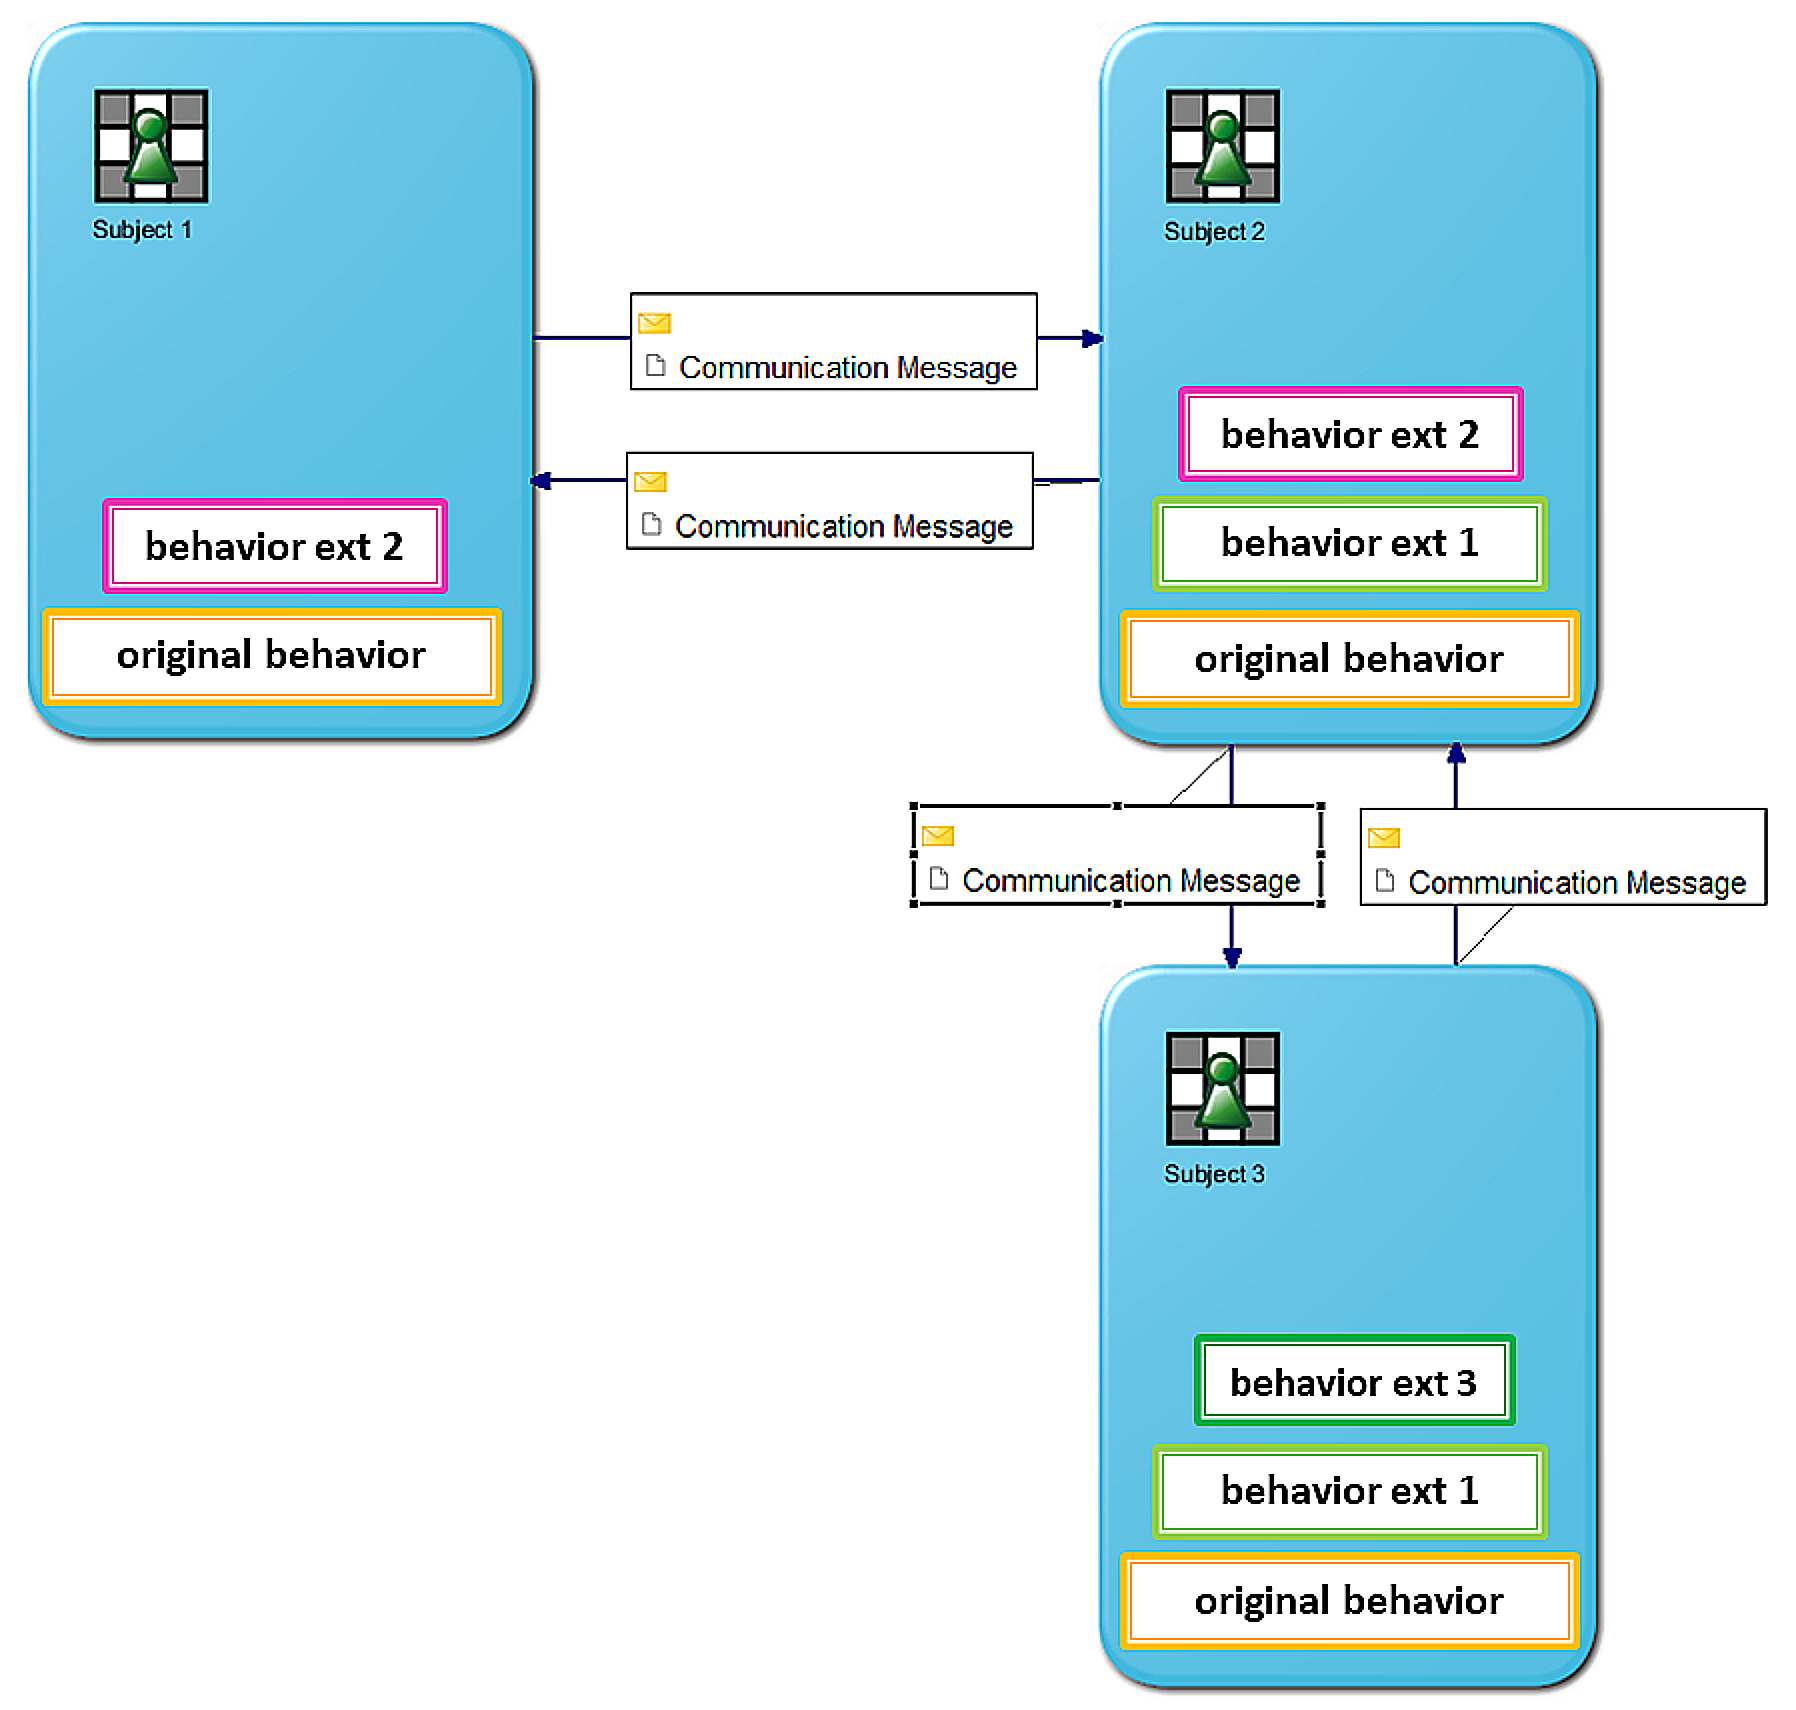
\includegraphics[width=0.8\linewidth]{Figures/Chapter5/ArbitratorPattern/ArbitratorMultiBehaviorSubjects.png}
	\caption[Multi-Behavior Subjects]{Multi-Behavior Subjects}
	\label{fig:multiBehaviorSubject}
\end{figure}


\subsection{The arbitrator pattern for PASS execution}

The idea is to use the Arbitrator Pattern as basis for a mechanism to allow dynamic adaption and multi-behavior execution within an instance in work flow management system for PASS.  Instead of Motors and Sensors, in the context of PASS, a Subject interacts with its environment  via the reception and sending of Messages which can be directed to other subjects (the environment). Furthermore, internal inputs (user choices or other computations that determine actions of a Subject) can, or rather should affect the priorities of behaviors (i.e.: can determine which behavior is executed).
The equivalent to the sensors of a robot here is a subject’s ‘message In-Box’. And instead of controlling motors, here the arbitrator grants a Subject-Behavior the right to access the message facilities – to receive and send messages. 
Consequently, the core concept here is not to handle a subject as single SBD-interpreter-machine, but rather as multiple interpreter machines encapsulated in an arbitrator-controlled-machine which can grant control rights for the unit/subject. Towards the outside a subject is in principle a single unit with its Message In-Box and outgoing messages. The original $BEHAVIOR(subj,state)$ ASM defined by Börger in \cite{boerger2011interpreter} needs to be adapted in order to really fit into the concept presented here. For now it is assumed that the definition will work. Under normal circumstances i there should be only one behavior container, containing a $BEHAVIORD(subj, state)-ASM$. For the arbitrator pattern to work, it is assumed to be encapsulated in a container which has a priority and execution functionality: 

{\newcommand\tab[1][1cm]{\hspace*{#1}}\begin{small}\begin{textit} \noindent  \\
$BEHAVIOR\_INTERPRETER\_CONTAINER(D, subj, state, containerID ) =$ \\
    \indent \textbf{seq} \\
    \indent \textbf{if} $couldTakeControl(D, subj,state)$ \textbf{then} \\
    \indent \tab $updatePriorityForArbitrator(subj, thisContainer)$ \\
    \indent \textbf{if} $hasControl(subj, containerID)$  \textbf{then} \\
    \indent \tab$BEHAVIORD(subj,state)$ \\
\end{textit}\end{small}}
\bigskip


This definition should express that, when executed, the behavior container checks whether it $couldTakeControl$ of the subject or not and updates the priorities. Based on that priority list the arbitrating machine will grant the access right via the take-Control command that should evaluate as true for the empowered $BEHAVIOR\_INTERPRETER\_CONTAINER$ machine. 
Upon a special change request – e.g. a special message (or event) outside the process context containing a new model ($behaviorExtensionArrived$) – the $ARBITRATOR(subj, context)$ can initialize and/or start a new interpreter machine based on the received model D to take control of the subject. The condition of course, and the need for further research, is that the new model data $isValidForContext(newestBehaviorDiagram(subj), processContext)$ in order to fit logically into the current process context which is given by the model the original behavior-machine is based on. The initialized machines need to be traced/collected in a location of $activeBehaviours(subj)$.The source of such a special message for now is assumed to be an administrator outside the process context. More elaborate or sophisticated mechanisms are imaginable.  By default a newer model simply has a higher priority for execution. Further rules to determine priority will be needed. 

An attempt to specify the described mechanism with the means of ASMs is given here:

{\newcommand\tab[1][1cm]{\hspace*{#1}}\begin{small}\begin{textit} \noindent  \\
$ARBITRATOR(subj, processContext)$ \\
    \indent\textbf{seq}\\
	\indent \textbf{if} $behaviorExtensionArrived(subj, processContext, D*)$ \textbf{then} \\
	\tab \textbf{if} $isValidForContext(newestBehaviorDiagram(subj), processContext)$ \textbf{then} \\		
         \indent \tab $initializeNewBehaviorInterpreterContainer(newestBehaviorDiagram(subj))$
	\indent \textbf{else} \textbf{forall}  i in activeBehaviours(subj) \textbf{do } \\
	     \tab  $hasControl(subj, i) := false$ \\
	     \tab $BEHAVIOR\_INTERPRETER\_CONTAINER(D, subj, state)$ \\
	  \indent \textbf{choose} j in $activeBehaviours(subj)$ \textbf{where} $priority(j) > priority(x){x != j}$ \\
	 	  \tab hasControl(subj, j) := true

\end{textit}\end{small}}
\bigskip

This machine should execute with a certain frequency, repeating the cycle and being aware of new behaviors, reevaluating priorities and (re-)granting control to a behavior continuously. In the case of the original robotics concept, behavior changes can occur in the span of milliseconds depending on the power and speed of the controlling computer. In a business process context, a behavior change may not need the strict real-time requirement since a change might not occur at all or only a few times in the span of, e.g., a minuet.

\subsection{Final Thoughts}

The proposed mechanism is not very complicated. In robotics this simple approach allows to construct complex behavior out of simple elements.  Our future research will be aimed at investigating whether the application of this concept here can be useful and to find possible drawbacks (e.g. validation concerns) and challenges that would need to be addressed before actual applying this concept. First of all being the definition of valid model extensions mechanism/validator rules for PASS, followed by issues like the priority determination and the question about frequency of priority updates and actual behavior changes among other details needed to actually build a prototypical implementation as the high goal. 

